%==============================================================================
%== template for LATEX poster =================================================
%==============================================================================
%
%--A0 beamer slide-------------------------------------------------------------
\documentclass[final]{beamer}
\usepackage[orientation=portrait,size=a0,
            scale=1.3         % font scale factor
           ]{beamerposter}
           
\geometry{
  hmargin=2.5cm, % little modification of margins
}

%
%\usepackage[T2A]{fontenc}
\usepackage[english, russian]{babel}
\usepackage[utf8]{inputenc}
\usepackage[default]{opensans}

\linespread{1.3}
%
%==The poster style============================================================
\usetheme{sharelatex}
\usepackage{lmodern}

%==Title, date and authors of the poster=======================================
\title
[III-ая Всероссийская школа НЦФМ по физике высоких энергий, ядерной физике и ускорительной технике] % Conference
{ % Poster title
ИССЛЕДОВАНИЕ СПИН-ОРБИТАЛЬНОЙ ДИНАМИКИ ДЛЯ ИССЛЕДОВАНИЯ ЭДМ В НАКОПИТЕЛЬНЫХ КОЛЬЦАХ
}

\author{ % Authors
Колокольчиков С., Сеничев Ю.
}
\institute
[Институт Ядерных Исследований РАН, Москва, Россия] % General University
{
Институт Ядерных Исследований РАН, Москва, Россия\\[0.3ex]
Московский физико-технический институт (НИУ), Долгопрудный, Россия
}
\date{\today}

\begin{document}
\begin{frame}[t]
%==============================================================================
\begin{multicols}{3}
%==============================================================================
%==The poster content==========================================================
%==============================================================================

\section{Барионная асимметрия}
Наблюдаемая барионная асимметрия, означает преобладание материи над антиматерией во Вселенной. В 1967 г. А. Сахаров теоретически установил, что необходимым условием для бариогенеза является нарушение CP-инвариантности \cite{ref1}.
\section{ЭДМ}

Существование ненулевых электрических дипольных моментов (ЭДМ) элементарных частиц нарушает CP-инвариантность и способно установить применимость теорий, выходящих за рамки Стандартной Модели (СМ) физики частиц \cite{ref2}

\begin{figure}[h]
            \centering
            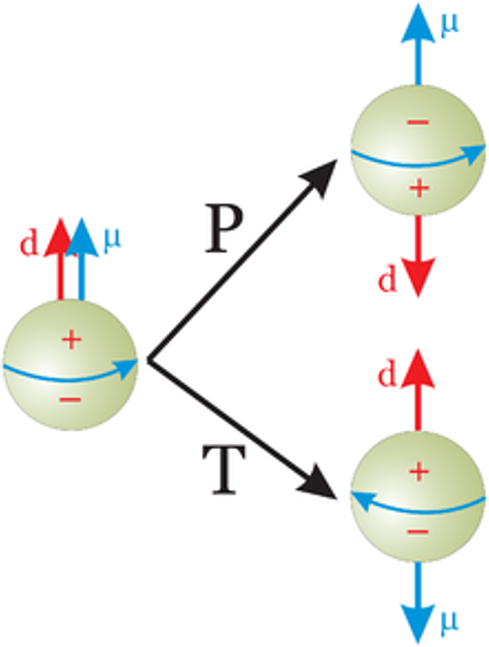
\includegraphics[height=.2\textheight]{EDM CP}
\end{figure}

\section{Т-БМТ уравнение}

Идея исследования ЭДМ частиц основана на уравнении Т-БМТ (Томас, Баргман, Мишель, Телегди) \cite{ref3}. Описывающего динамику классического спин-вектора для ансамбля частиц. 

\begin{equation}
\begin{aligned}
\frac{d \vec{S}}{d t} & =\vec{S} \times\left(\vec{\Omega}_{M D M}+\vec{\Omega}_{E D M}\right), \\
\vec{\Omega}_{M D M} & =\frac{q}{m \gamma}\left\{(\gamma G+1) \vec{B}_{\perp}+(G+1) \vec{B}_{\|}-\right. \\
& \left.-\left(\gamma G+\frac{\gamma}{\gamma+1}\right) \frac{\vec{\beta} \times \vec{E}}{c}\right\}, \\
\vec{\Omega}_{E D M} & =\frac{q \eta}{2 m}\left(\vec{\beta} \times \vec{B}+\frac{\vec{E}}{c}\right), \quad G=\frac{g-2}{2},
\end{aligned}
\end{equation}

Вращение происходит в результате взаимодействия внешних магнитного и электрического поля с магнитным и электрическим дипольным моментами (МДМ и ЭДМ).
\newline
\newline
\newline
\newline
\section{Накопительные кольца}

Для заряженных частиц, протонов и дейтронов, необходимо использование кольцевых накопительных установок. Первоначально была предложена концепция «замороженного спина» \cite{ref4}. В настоящее время разрабатывается концепция накопителя ProtoType Ring (PTR) специально для поиска ЭДМ дейтронов и протонов \cite{ref5}.
\begin{figure}[h]
            \centering
            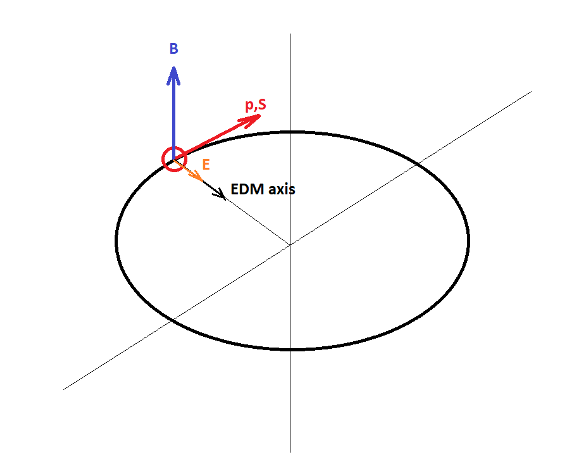
\includegraphics[height=.2\textheight]{FS.png}
\end{figure}

\begin{figure}[h]
            \centering
            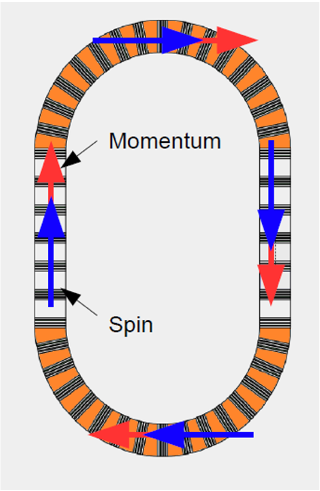
\includegraphics[height=.2\textheight]{FS ring.png}
\end{figure}

\section{Комплекс NICA–Nuclotron}

В России исследование поляризованного пучка дейтронов может быть осуществлено при помощи концепции «квази-замороженного спина» на коллайдере NICA, Дубна \cite{ref6} и модернизированной структуре Nuclotron, бустером в коллайдер \cite{ref7}.

\begin{figure}[h]
            \centering
            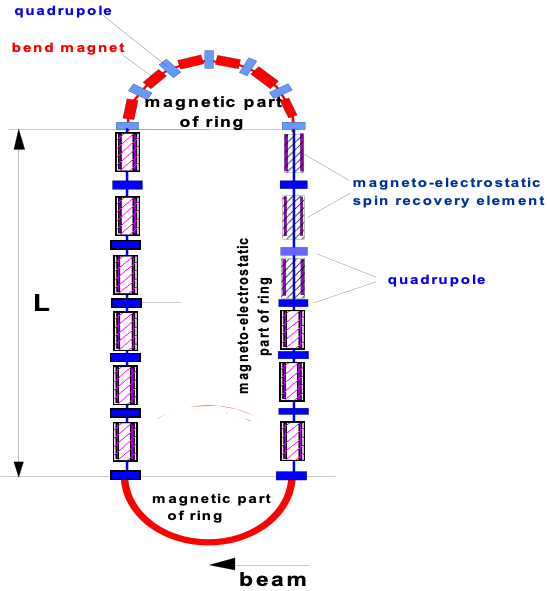
\includegraphics[height=0.2\textheight]{QFS ring.png}
\end{figure}

\section{Задачи}

\begin{itemize}
    \item Реализация «квази-замороженного» спина;
    \item Достижение максимального время спиновой когерентности (SCT) частиц в сгустке более 1000 с.;
    \item Обеспечение точности измерения частоты прецессии спина;
    \item Оценка вклада систематических ошибок в общую частоту прецессии спина должен быть меньше, чем вклад сигнала от ЭДМ.
\end{itemize}


%==============================================================================
%==End of content==============================================================
%==============================================================================

%--References------------------------------------------------------------------

\section{Литература}

\begin{thebibliography}{99}

\bibitem{ref1} A. D. Sakharov, Violation of CP in variance, С asymmetry, and baryon asymmetry of the universe, Pis’maZh. Eksp.Teor. Fiz. 5,32-35 (1967), \textit{JETPLett.} 5,24-27 (1967),DOI:10.1070/PU1991v034n05ABEH002497

\bibitem{ref2} D. Anastassopoulos, et al., AGS Proposal: Search for a permanent electric dipole moment of the deuteron nucleus at the 10-29 e cm level, April, 2008.

\bibitem{ref3} V. Bargmann, Louis Michel, and V. L. Telegdi Precession of the Polarization of Particles Moving in a Homogeneous Electromagnetic Field, \textit{Phys. Rev. Lett.} 2, 435, DOI: https://doi.org/10.1103/PhysRevLett.2.435 
\bibitem{ref4} F. J.M. Farley, K. Jungmann, J.P. Miller, W.M. Morse, Y.F. Orlov, B. L. Roberts, Y.K. Semertzidis, A. Silenko, and E. J. Stephenson, \textit{Phys. Rev. Lett.} 93, 052001 (2004). 
\bibitem{ref5} F. Abusaif, A. Aggarwal, A. Aksentev et al. (CPEDM collaboration), \textit{CERN Yellow Reports: Monographs}, 2021-003, CERN, Geneva (2021).
\bibitem{ref6} Quasi-frozen spin concept of magneto-optical structure of NICA adapted to study the electric dipole moment of the deuteron and to search for the axion, Y. Senichev, A. Aksentyev, S. Kolokolchikov, A. Melnikov, V. Ladygin, E. Syresin and N. Nikolaev, \textit{Journal of Physics: Conference Series}, 2420 (2023) 012052, doi:10.1088/1742-6596/2420/1/012052
\bibitem{ref7} Senichev, Y.V., Aksentyev, A.E., Kolokolchikov, S.D. et al. Consideration of an Adapted Nuclotron Structure for Searching for the Electric Dipole Moment of Light Nuclei. \textit{Phys. Atom. Nuclei} 86, 2434–2438 (2023). https://doi.org/10.1134/S1063778823110418

\end{thebibliography}
%--End of references-----------------------------------------------------------

\end{multicols}

%==============================================================================
\end{frame}
\end{document}
